\documentclass[fleqn]{jbook}
\usepackage{physpub}

\begin{document}

\begin{question}{専攻 問題2}{}

長さ$L$,半径$b$の金属パイプ(抵抗はゼロとする)の中心軸に沿って半径$a$,長さ
$\ell$の荷電粒子群が速度$v$で通過する。荷電粒子群内での線電荷密度(単位長さあ
たりの電荷量)$\sigma$は一様であるとする。金属パイプは,図に示すように,容量
$C$および抵抗$R$を通じて接地されており,抵抗$R$の両端間の電位差$V$の時間変化
をオシロスコープ上で観測するものとする。

\begin{subquestions}
\SubQuestion
 荷電粒子群が周期$T$で繰り返し金属パイプ内を同一方向に通過するとき,パイ
プの内壁面に静電誘導される電荷量$Q(t)$を求め,横軸を時間軸にとって図示せよ。
ただし,$\ell\gg L \quad ,\quad T\gg\ell/v$とする。

\SubQuestion
 金属パイプの外壁につながる容量$C$のコンデンサー上には,電荷量$Q_c(t)$が
現れる。そのとき$Q(t)$と$Q_c(t)$および抵抗を流れる電流$j(t)$との関係式を求め
よ。また,電圧$V(t)$の満たすべき微分方程式を求めよ。

\SubQuestion
 誘導電荷量$Q(t)$および電圧$V(t)$を次のようにスペクトル分解するとき,
電圧$V(t)$のスペクトル成分$\hat{V}(\omega)$を,設問(2)の$V(t)$の式を用いて
$\hat{Q}(\omega)$の関数として求めよ。角周波数$\omega$に対する$\hat{V}(\omega)$
の絶対値$|\hat{V}(\omega)|$の概略図を,$\omega=0$近傍に注目して描け。
\[Q(t)=\int_0^{\infty}\hat{Q}(\omega)e^{i\omega t}d\omega,
\hspace{5mm} V(t)=\int_0^{\infty}\hat{V}(\omega)e^{i\omega t}d\omega \]

\SubQuestion
設問{\bf{2}}において求めた$V(t)$の微分方程式の解を求め,以下の場合にオシロス
コープ(入力インピーダンスは$\rm 1M\Omega$とする)上で観測される電圧波形の概
略を図示せよ。
\begin{eqnarray*}
&&R=100{\rm k\Omega},\hspace{5mm}C=1\times10^{-9}{\rm Farad},
\hspace{5mm}\ell=30{\rm m},\hspace{5mm}L=0.3{\rm m},\hspace{5mm}
v=3\times10^7{\rm m/sec} \\
&& 長さ\ell に含まれる荷電粒子数: N=1\times10^{10}個,
粒子の電荷:e=1.6\times10^{-19}{\rm Coulomb} 
\end{eqnarray*}
また,抵抗$R$を$50\Omega$とした場合はどのような波形となるか。
\end{subquestions}
\begin{center}
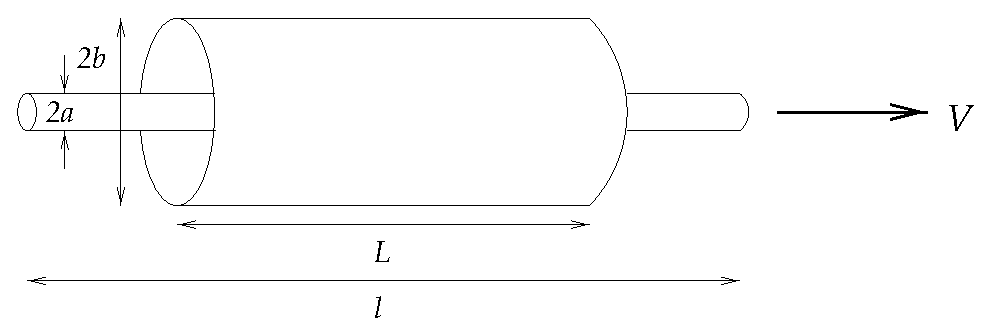
\includegraphics[clip,height=25mm,width=80mm]{1992phy2-0.eps}

\vspace{5mm}
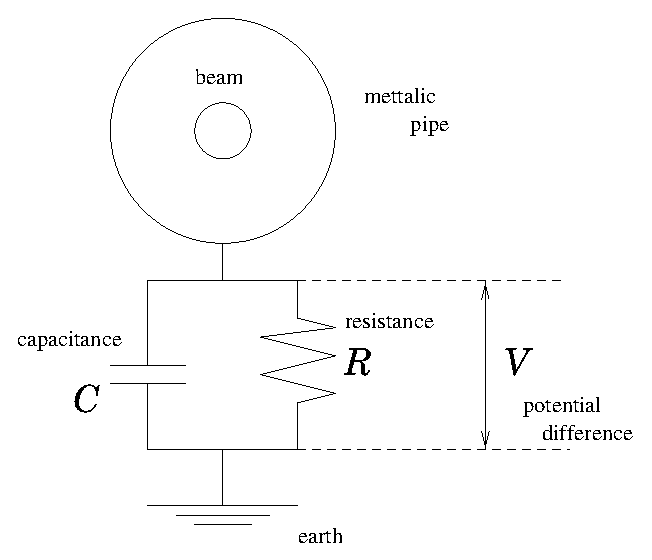
\includegraphics[clip,height=45mm,width=50mm]{1992phy2-1-2.eps}
\end{center}

\end{question}
\begin{answer}{専攻 問題2}{}
\begin{subanswers}

\SubAnswer
\parbox[t]{85mm}{
この問いに厳密に答えるのは非常に難しい。そこで単に円筒形コンデンサーの問題
として考えれば十分と思われる(この仮定は、回路の緩和時間$RC$が、粒子群がパイプ
を横切る時間$L/v$に対して十分長ければ妥当である)。

粒子群がパイプ内にある時、パイプ内壁に静電誘導される電荷量は$-\sigma L$である。
そして、粒子群がパイプ内を完全に横切るのにかかる時間は$(L+\ell)/v\simeq \ell/v$
である。従って$Q(t)$の時間変化は右図のようになる。
}\parbox[t]{60mm}{\vspace{-10mm}
\begin{center}
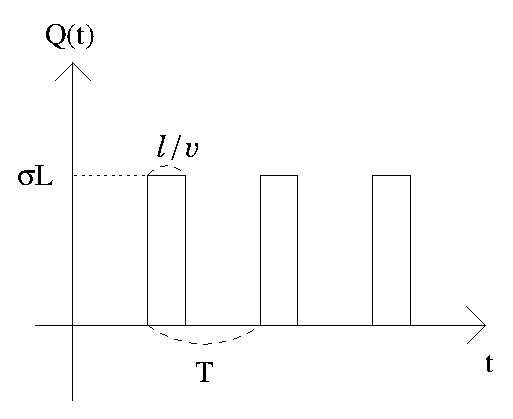
\includegraphics[clip,height=50mm,width=60mm]{1992phy2-1-1.eps}
\end{center}
}
\SubAnswer
\parbox[t]{95mm}{
図のように$Q_{c}$と$j$の符号を定める。すると、
\begin{eqnarray}
&&\frac{d}{dt}\left( Q(t)+Q_{c}(t)\right) =j(t) \eqname{A1}\\
&&V(t)=-Rj(t)=\frac{1}{C}Q_{c}(t) \eqname{A2}
\end{eqnarray}
がなり立つ。\eqhref{A2}を用いて\eqhref{A1}から$j,Q_{c}$を消去すると、
\begin{equation}
\frac{dV(t)}{dt}+\frac{1}{RC}V(t)=-\frac{1}{C}\frac{dQ(t)}{dt} \eqname{A3}
\end{equation}
となる。
}\parbox[t]{50mm}{\vspace{-10mm}
\begin{center}
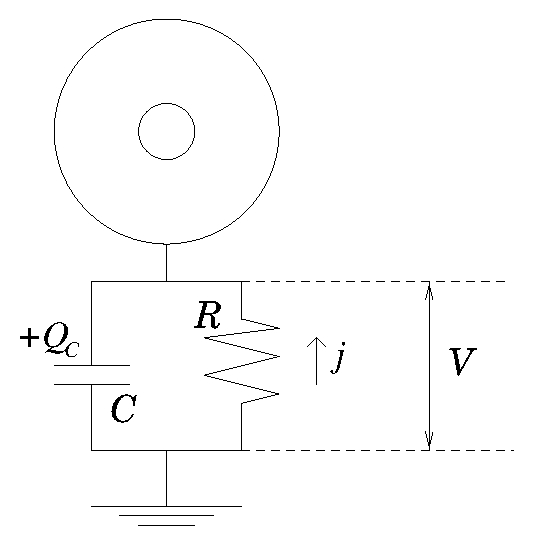
\includegraphics[clip,height=45mm,width=45mm]{1992phy2-1-3.eps}
\end{center}
}

\SubAnswer
問題文では積分の下限が$0$になっている。この理由が私には良く分からない。問題文
のままでは$Q(t)$が実数であることを保証できないように思うのだが…。

以下ではとりあえず通常のフーリエ変換を用いて設問に答えることにする(今
繰り返しの周期$T$は十分に長いとしているので、フーリエ級数でもフーリエ変換でも
同じ結果になる)
\begin{equation}
V(t)=\int_{-\infty}^{\infty}\tilde{V}(\omega)e^{i\omega t}d\omega \quad , \quad 
Q(t)=\int_{-\infty}^{\infty}\tilde{Q}(\omega)e^{i\omega t}d\omega \eqname{A4}
\end{equation}
式\eqhref{A4}を式\eqhref{A3}に代入し、各周波数成分毎にまとめると
\begin{eqnarray}
i \omega \tilde{V}(\omega)+\frac{1}{RC}\tilde{V}(\omega)&=&-\frac{i\omega}{C}
\tilde{Q}
(\omega)\nonumber\\
\Yueni \quad \tilde{V}(\omega)=-\frac{i\omega}{\frac{1}{RC}+i\omega}\frac{\tilde{Q}(\omega)}{C} \eqname{A5}
\end{eqnarray}
となる。今$Q(t)$を$0\le t \le \ell/v$で$-\sigma L$、それ以外で$0$とすると
$\tilde{Q}(\omega)$は、
\[
\tilde{Q}(\omega)=\frac{1}{2\pi}\int_{-\infty}^{\infty}Q(t)e^{-i\omega t}dt
=\frac{1}{2\pi}\int_{0}^{\ell /v}(-\sigma L)e^{-i\omega t}dt
=\frac{\sigma L}{2\pi}\frac{e^{-i\omega \ell /v}-1}{i\omega}
\]
となる。したがって$\tilde{V}(\omega)$は、

\begin{eqnarray}
\tilde{V}(\omega)&=&-\frac{1}{2\pi}\frac{e^{-i\omega \ell /v}-1}{\frac{1}
{RC}+i\omega}\frac{\sigma L}{C} \eqname{A6}\\
よって\hspace{1cm}
|\tilde{V}(\omega)|&=&\frac{1}{\pi}\left|\frac{\sigma L}{C}\right|
\frac{|\sin 
\frac{\omega \ell}{2v}|}{\sqrt{\left( \frac{1}{RC}\right) ^{2}+\omega ^{2}}}
\sim \frac{RC}{\pi}\left|\frac{\sigma L}{C}\right|\left|
\frac{\omega \ell}{2v}\right|\hspace{5mm}(ただし、\omega 
\simeq 0)\nonumber
\end{eqnarray}
となる。$|\tilde{V}(\omega)|$の概略図は次の通りになる。

\begin{center}
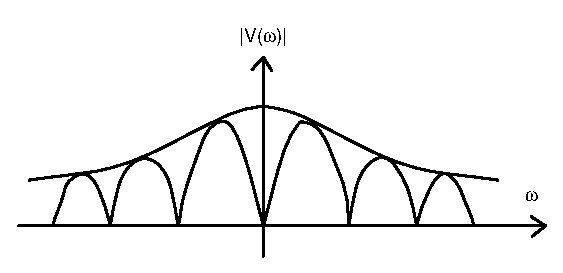
\includegraphics[clip]{1992phy2-2.eps}
\end{center}

\SubAnswer

式\eqhref{A6}を積分して$V(t)$を求める
($V(t)$を求めるだけなら、式\eqhref{A3}を定数変化法で解くこともできる)。
\begin{eqnarray*}
V(t)&=&\int_{-\infty}^{\infty}\tilde{V}(\omega)e^{i\omega t}d\omega\\
&=&-\frac{1}{2\pi}\frac{\sigma L}{C}\left\{\int_{-\infty}^{\infty}\frac
{e^{i\omega(t-\ell /v)}}{\frac{1}{RC}+i\omega}d\omega-\int_{-\infty}^{\infty}
\frac{e^{i\omega t}}{\frac{1}{RC}+i\omega}d\omega\right\}\\
&=&\left\{
\begin{array}{ll}
0,& \quad (t<0)\\
\frac{\sigma L}{C}e^{-\frac{t}{RC}},& \quad (0<t<\ell /v)\\
\frac{\sigma L}{C}e^{-\frac{t}{RC}}(-e^{\frac{\ell /v}{RC}}+1),& \quad (t>\ell /v)\\
\end{array}\right.
\end{eqnarray*}
問題文で与えられた値を代入すると、
\begin{eqnarray*}
\frac{\sigma L}{C}&=&\frac{1}{C}\frac{eN}{\ell}L=1.6\times 10^{-2}[{\rm V}]\\
\frac{\ell}{v}&=&10^{-6}[{\rm sec}]\\
RC&=&\left\{
\begin{array}{ll}
10^{-4}[{\rm sec}]& \quad (R=100{\rm k}\Omega)\\
5\times 10^{-8}[{\rm sec}]& \quad (R=50\Omega)\\
\end{array} \right.
\end{eqnarray*}
となる。ただしオシロスコープの入力インピーダンスは十分大きいので影響を
無視した。

オシロスコープで観測される波形は下図のようになる。
\begin{center}
\includegraphics[clip]{1992phy2-3.eps}
\end{center}
\end{subanswers}
\end{answer}



\end{document}